\item Find the area bounded by the lines $3x+2y=14$, $2x-3y=5$ in the first quadrant.

\hfill{(IN 2016)}
\begin{enumerate}
\begin{multicols}{4}
\item 14.95
\item 15.25
\item 15.70
\item 20.35
\end{multicols}
\end{enumerate}
\item A straight line of the form $y = mx + c$ passes through the origin and the point \brak{x, y} = \brak{2, 6}. The value of $m$ is \rule{2cm}{0.4pt}.
\hfill{(IN 2016)}
\item The vector that is NOT perpendicular to the vectors \brak{i + j + k} and \brak{i + 2j + 3k} is 
\hfill{(IN 2016)}
\begin{enumerate}
\begin{multicols}{4}
\item \brak{i-2j+k}
\item \brak{-i + 2j-k}
\item \brak{0i + 0j + 0k}
\item \brak{4i +3 j + 5k}
\end{multicols}
\end{enumerate}
\item The signal $x\sbrak{n}$ shown in \figref{fig:z4} is convolved with itself to get $y\sbrak{n}$. The value of $y\sbrak{-1}$ is \rule{2cm}{0.4pt}.
\hfill{(IN 2016)}
\begin{figure}[H]
\centering
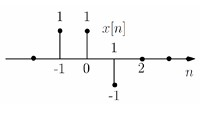
\includegraphics[width=0.5\columnwidth]{GATE/2016/IN/figs/z4.jpg}
\caption{}
\label{fig:z4}
\end{figure}
\item Consider the matrix
\begin{align*}
\vec{A} = \myvec{2 & 1 & 1 \\ 2 & 3 & 4 \\ -1 & -1 & -2}
\end{align*}
whose eigenvalues are $1, -1$ and $3$. Then Trace of $\brak{\vec{A}^3 - 3\vec{A}^2}$ is \rule{1cm}{0.01pt}.
\hfill{(IN 2016)}
